\section{条件期望的定义}
\label{sec:cexp-definition}

第~\ref{chap:random-vectors}章的条件均值都靠除法得到：组内的累计期望除以这一组的概率。只要组的概率为正，这个除法就有意义；一旦条件事件的概率为零，或者根本没有概率表和密度，它就失效。这一节先把有限分组的组内平均重新写成一个随机变量，找出它满足的两条性质；再把这两条性质当作定义，使它在分组概率为零时依然有意义；然后证明这样的随机变量存在而且几乎必然唯一；最后回到给定一个观测的情形，说明条件平均为什么是观测值的函数。

\subsection{有限分组中的条件平均}
\label{sec:cexp-finite-partition}

\paragraph{把组内平均写成随机变量}
回到两台传感器。第一台的档位为$X$，第二台为$Y$，联合概率表见图~\ref{fig:cexp-sensor-rows}(a)。把表中九个格子看作样本空间$\Omega$的九个样本点，每个格子的概率就是表中的数，其中$(0,2)$与$(2,0)$两格的概率为零。$X$与$Y$是这九个点上的函数：格子$(x,y)$上$X=x$，$Y=y$。

\begin{BookInlineFigure}
  \centering
  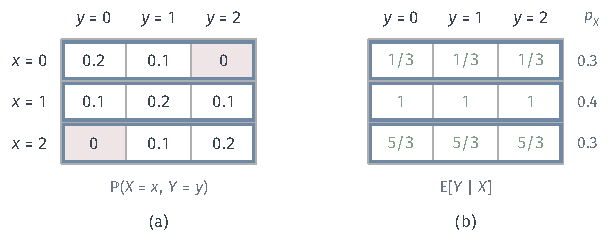
\includegraphics[width=104mm]{figures/07-probability/02-measure-theoretic-probability/tikz/cexp-sensor-rows/figure.pdf}
  \caption{传感器表上的组内平均。(a)九个格子组成样本空间，格中是概率，浅红格的概率为零；蓝框是按$X$的取值分成的三组。(b)随机变量$\mathbb{E}[Y\mid X]$：同一行的每个格子都取这一行$Y$的平均$1/3$、$1$、$5/3$，右侧是各行的概率$p_X$。}
  \label{fig:cexp-sensor-rows}
\end{BookInlineFigure}

知道$X$的值，相当于知道样本点落在哪一行。第~\ref{chap:random-vectors}章算出三行的条件均值$m(0)=1/3$、$m(1)=1$、$m(2)=5/3$。把这三个数填回格子，每一行的所有格子都填该行的均值，就得到图~\ref{fig:cexp-sensor-rows}(b)：一个定义在$\Omega$上的新函数，也就是随机变量$m(X)$。它在样本点$\omega$处的值，是“与$\omega$同组的所有样本点上$Y$的平均”。这个随机变量记作$\mathbb{E}[Y\mid X]$。

这样看，条件平均有两种身份。$m(x)$是一个数，回答“已知$X=x$时$Y$平均是多少”；$\mathbb{E}[Y\mid X]$是一个随机变量，回答“在还不知道结果时，按将来会得到的信息所作的平均是什么”。后者把三个问题的答案一次装进一个对象，本章研究的正是这个对象。

\paragraph{一般的有限分组}
分组不必按某个变量的取值进行。设事件$A_1,\dots,A_k$两两不交，并起来是$\Omega$，称为$\Omega$的一个有限划分。知道“样本点落在哪一组”，就能判断由若干组并成的任何事件是否发生；把这些并集合起来（包括空集），得到
\[
 \mathcal{G}=\Bigl\{\textstyle\bigcup_{i\in S}A_i:\ S\subseteq\{1,\dots,k\}\Bigr\},
\]
它恰好有$2^{k}$个事件。$\mathcal{G}$对补和并封闭，是一个$\sigma$代数，并且是包含$A_1,\dots,A_k$的最小$\sigma$代数。第~\ref{chap:probability-spaces}章用$\sigma$代数表示观测所能区分的信息，$\mathcal{G}$就是“知道所在组”这份信息。按$X$分行时，$\mathcal{G}=\sigma(X)$。

对可积的随机变量$X$，在每个概率为正的组内求平均，再把平均值赋给该组的所有样本点，就得到有限划分下的条件期望：
\begin{equation}
 \mathbb{E}[X\mid\mathcal{G}]=\sum_{i=1}^{k}c_i\mathbf{1}_{A_i},\qquad
 c_i=\frac{\mathbb{E}[X\mathbf{1}_{A_i}]}{\mathbb{P}(A_i)}\quad\text{当}\ \mathbb{P}(A_i)>0 .
 \label{eq:cexp-partition}
\end{equation}
$c_i$正是第~\ref{chap:classical-probability}章“缩小样本范围再重新归一”的平均：把$X$限制在$A_i$上求期望，再除以$A_i$的概率。$\mathbb{P}(A_i)=0$的组没有可以除的数，$c_i$任取一个常数。

\paragraph{概率为零的组}
按读数之差$D=X-Y$分组，就会遇到这种组。$D$取$-2,-1,0,1,2$五个值，对应传感器表的五条对角线，见图~\ref{fig:cexp-difference-groups}(a)。$D=2$与$D=-2$各只含一个概率为零的格子：两台读数从不相差两档。

\begin{BookInlineFigure}
  \centering
  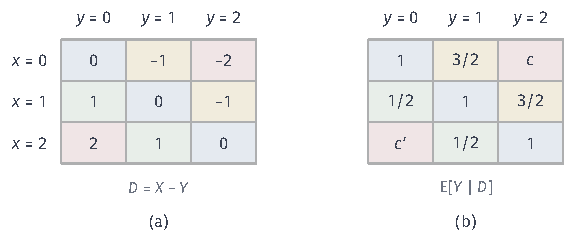
\includegraphics[width=96mm]{figures/07-probability/02-measure-theoretic-probability/tikz/cexp-difference-groups/figure.pdf}
  \caption{按读数之差$D=X-Y$分组。(a)每个格子所属的组，同色格子同组；浅红的两组$D=\pm2$概率为零。(b)$\mathbb{E}[Y\mid D]$在三组正概率组上分别取$1$、$1/2$、$3/2$，在两个零概率组上取任意常数$c$、$c'$。}
  \label{fig:cexp-difference-groups}
\end{BookInlineFigure}

由式~\eqref{eq:cexp-partition}逐组计算。$D=0$的三个格子概率都是$0.2$，$Y$分别取$0,1,2$；$D=1$的两个格子是$(1,0)$与$(2,1)$，概率都是$0.1$；$D=-1$的两个格子是$(0,1)$与$(1,2)$。于是
\[
 \begin{gathered}
 c_{D=0}=\frac{0.2\cdot(0+1+2)}{0.6}=1,\\
 c_{D=1}=\frac{0.1\cdot(0+1)}{0.2}=\frac12,\qquad
 c_{D=-1}=\frac{0.1\cdot(1+2)}{0.2}=\frac32 .
 \end{gathered}
\]
两台读数一致时，第二台的平均档位是$1$；第一台比第二台高一档时，第二台偏低，平均$1/2$；反过来平均$3/2$。$D=\pm2$两组上的值没有可算的依据，图~\ref{fig:cexp-difference-groups}(b)记作$c$与$c'$。

\paragraph{两条性质}
式~\eqref{eq:cexp-partition}得到的随机变量$Z=\mathbb{E}[X\mid\mathcal{G}]$有两条性质，它们后面会变成定义。

第一条，$Z$在每一组内取常数，所以只用到“所在组”这份信息。用$\sigma$代数的语言说：对任何实数集合$B$，$\{Z\in B\}$是若干整组的并，属于$\mathcal{G}$，即$Z$是$\mathcal{G}$可测的。反过来，一个$\mathcal{G}$可测的函数也必定在每组内取常数，因为单点集的原像$\{Z=z\}$只能是整组的并。

第二条，$Z$在每个已知事件上保留$X$的累计期望：
\[
 \mathbb{E}[Z\mathbf{1}_{A}]=\mathbb{E}[X\mathbf{1}_{A}],\qquad A\in\mathcal{G}.
\]
证明只需逐组核对。$A$是若干组$A_i$的并，两边都按组拆成和。对$\mathbb{P}(A_i)>0$的组，由$c_i$的定义，
\[
 \mathbb{E}[Z\mathbf{1}_{A_i}]=c_i\,\mathbb{P}(A_i)=\mathbb{E}[X\mathbf{1}_{A_i}] .
\]
对$\mathbb{P}(A_i)=0$的组，$\mathbf{1}_{A_i}$只在零概率集上非零，两边都是$0$，与$c_i$怎样选无关。把各组相加，就得到上式。

用$D$分组核对一次。取$A=\{D=0\}\cup\{D=1\}$。$Y$在这五个格子上的累计期望为
\[
 \mathbb{E}[Y\mathbf{1}_{A}]=0.2\cdot(0+1+2)+0.1\cdot(0+1)=0.7 ,
\]
而$Z=\mathbb{E}[Y\mid D]$在其中三格取$1$、两格取$1/2$，
\[
 \mathbb{E}[Z\mathbf{1}_{A}]=1\cdot0.6+\tfrac12\cdot0.2=0.7 .
\]
若把$A$换成含有零概率组的事件，例如再并上$\{D=2\}$，两边都不变，$c'$的取值不起作用。

\paragraph{连续样本空间上的有限分组}
样本空间本身不必有限。取$\Omega=[0,1)$，概率是区间长度，令$X(\omega)=\omega^{2}$。把$[0,1)$等分成$2^{n}$段，记这些区间生成的$\sigma$代数为$\mathcal{G}_n$，它表示“只知道$\omega$落在哪一段”。每段的概率为$2^{-n}>0$，式~\eqref{eq:cexp-partition}直接适用。区间$[a,b)$上的平均为
\[
 \frac{1}{b-a}\int_{a}^{b}\omega^{2}\,\mathrm{d}\omega=\frac{a^{2}+ab+b^{2}}{3}.
\]

取$n=2$，四段是$[0,\tfrac14)$、$[\tfrac14,\tfrac12)$、$[\tfrac12,\tfrac34)$、$[\tfrac34,1)$，代入上式，例如第二段为$(\tfrac1{16}+\tfrac18+\tfrac14)/3=\tfrac{7}{48}$，四段依次得到
\[
 \tfrac{1}{48},\qquad \tfrac{7}{48},\qquad \tfrac{19}{48},\qquad \tfrac{37}{48}.
\]
$\mathbb{E}[X\mid\mathcal{G}_2]$是取这四个值的阶梯函数，见图~\ref{fig:cexp-dyadic-average}(a)。在每一段内，阶梯下方的面积与抛物线下方的面积相等，浅蓝的两块“多出”与“缺少”的面积互相抵消，这正是第二条性质在单个组上的样子。分得越细，阶梯越贴近$X$，见图~\ref{fig:cexp-dyadic-average}(b)：信息越多，条件平均保留的$X$的细节越多。

\begin{BookInlineFigure}
  \centering
  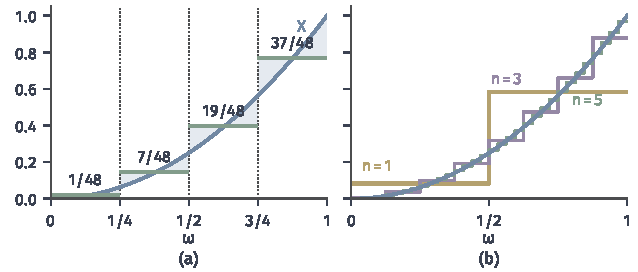
\includegraphics[width=108mm]{figures/07-probability/02-measure-theoretic-probability/matplotlib/cexp-dyadic-average/figure.pdf}
  \caption{$\Omega=[0,1)$上的均匀概率，$X(\omega)=\omega^{2}$（蓝）。(a)$\mathcal{G}_2$由四个等长区间生成，$\mathbb{E}[X\mid\mathcal{G}_2]$（绿）在各段取段内平均；每段内抛物线与阶梯之间的两块浅蓝面积相等。(b)$n=1$（黄）、$n=3$（紫）、$n=5$（绿）时的$\mathbb{E}[X\mid\mathcal{G}_n]$。}
  \label{fig:cexp-dyadic-average}
\end{BookInlineFigure}

\subsection{积分刻画}
\label{sec:cexp-integral}

\paragraph{分组的概率为零时}
回到章首的例子。取$\Omega=(-1,1)$，概率为长度的一半，令$X(\omega)=\omega$，于是$X\sim\operatorname{Unif}(-1,1)$；观测是$Y=\lvert X\rvert$。知道$Y$，就知道样本点在$\{\omega,-\omega\}$这一对之中，所以$\sigma(Y)$把$\Omega$分成不可数多个两点组，每组概率为零。式~\eqref{eq:cexp-partition}一个组也用不上。

直觉的答案是：同组两点概率对称，组内平均就是两点上函数值的算术平均。对正部$X^{+}$，在$\{\omega,-\omega\}$上的两个值是$\lvert\omega\rvert$与$0$，平均为$\lvert\omega\rvert/2$，所以候选答案是
\[
 Z=\frac{Y}{2}=\frac{\lvert X\rvert}{2}.
\]
图~\ref{fig:cexp-folding}(a)画出了它：红色虚线连接$\omega=\pm0.6$处的$X^{+}$，两端的平均$0.3$被赋给这两个点。

\begin{BookInlineFigure}
  \centering
  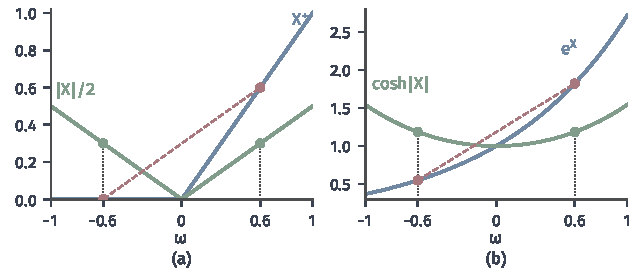
\includegraphics[width=108mm]{figures/07-probability/02-measure-theoretic-probability/matplotlib/cexp-folding/figure.pdf}
  \caption{只知道绝对值时的条件平均，$\Omega=(-1,1)$，$X(\omega)=\omega$均匀分布。(a)$X^{+}$（蓝）与候选的$\mathbb{E}[X^{+}\mid\lvert X\rvert]=\lvert X\rvert/2$（绿）；红点是同组的$\omega=\pm0.6$，两个函数值的平均$0.3$赋给这两点（绿点）。(b)同样地，$\mathrm{e}^{X}$（蓝）的组内平均是$\cosh\lvert X\rvert$（绿）。}
  \label{fig:cexp-folding}
\end{BookInlineFigure}

这个候选不能靠除法检验，但可以用上一小节的第二条性质检验。$\sigma(Y)$中的事件都形如$\{Y\in B\}$，$B\subseteq[0,1)$。$X$的密度在$(-1,1)$上是$\tfrac12$，于是
\[
 \mathbb{E}\bigl[X^{+}\mathbf{1}_{\{Y\in B\}}\bigr]
 =\int_{-1}^{1}\max(x,0)\,\mathbf{1}_{B}(\lvert x\rvert)\,\frac{\mathrm{d}x}{2}
 =\frac12\int_{0}^{1}x\,\mathbf{1}_{B}(x)\,\mathrm{d}x .
\]
另一边，$\lvert x\rvert/2$在$\pm x$处取同一个值，把$(-1,0)$与$(0,1)$两半合并，
\[
 \mathbb{E}\Bigl[\frac{Y}{2}\mathbf{1}_{\{Y\in B\}}\Bigr]
 =\int_{-1}^{1}\frac{\lvert x\rvert}{2}\,\mathbf{1}_{B}(\lvert x\rvert)\,\frac{\mathrm{d}x}{2}
 =\frac12\int_{0}^{1}x\,\mathbf{1}_{B}(x)\,\mathrm{d}x .
\]
两边对每个$B$都相等。候选答案在每个已知事件上保留了$X^{+}$的累计期望，尽管没有一个组可以单独拿来做除法。

\paragraph{定义}
这个例子说明，“在已知事件上保留累计期望”不需要除以组的概率，可以直接拿来作定义；再配上“只用已知信息”这一条，就把有限划分的情形推广到任意的信息。下面固定概率空间$(\Omega,\mathcal{F},\mathbb{P})$和一个$\sigma$代数$\mathcal{G}\subseteq\mathcal{F}$，$\mathcal{G}$表示已知的信息。

\begin{definition}[条件期望]
\label{def:cexp-conditional-expectation}
设$X$是可积的实随机变量，$\mathcal{G}\subseteq\mathcal{F}$是$\sigma$代数。若随机变量$Z$满足：
\begin{enumerate}
 \item $Z$是$\mathcal{G}$可测的；
 \item $Z$可积；
 \item 对每个$A\in\mathcal{G}$，
 \begin{equation}
  \mathbb{E}[Z\mathbf{1}_{A}]=\mathbb{E}[X\mathbf{1}_{A}],
  \label{eq:cexp-defining}
 \end{equation}
\end{enumerate}
则称$Z$为$X$给定$\mathcal{G}$的\term{条件期望}（conditional expectation），记作$\mathbb{E}[X\mid\mathcal{G}]$。满足要求的$Z$可能不止一个，其中每一个都称为\term{条件期望的版本}（version of a conditional expectation）。
\end{definition}

三条要求各有分工。$\mathcal{G}$可测限制了$Z$能用的信息：对每个Borel集$B$，“$Z\in B$是否发生”都必须能由已知事件判断，有限划分时这就是“组内取常数”。可积保证式~\eqref{eq:cexp-defining}左边有意义。式~\eqref{eq:cexp-defining}本身保证每个已知群体的平均不变：当$\mathbb{P}(A)>0$时两边同除以$\mathbb{P}(A)$，它说$Z$与$X$在$A$上的平均相同。

两种极端情形有助于看清定义。若$\mathcal{G}=\{\emptyset,\Omega\}$，什么也不知道，$\mathcal{G}$可测的随机变量只有常数，式~\eqref{eq:cexp-defining}对$A=\Omega$给出常数等于$\mathbb{E}[X]$，所以$\mathbb{E}[X\mid\mathcal{G}]=\mathbb{E}[X]$。若$X$本身是$\mathcal{G}$可测的，什么都已知道，$Z=X$满足全部三条，$\mathbb{E}[X\mid\mathcal{G}]=X$。一般情形介于两者之间：$Z=X$保留了所有累计期望，但通常用了未知的信息；常数$\mathbb{E}[X]$只用已知信息，但只在$A=\Omega$上保留累计期望。条件期望是满足这两方面要求的随机变量。

\paragraph{用定义检验候选}
定义并不给出计算公式，它的作用是检验：先由结构猜出候选，再验证三条要求。用第~\ref{chap:random-vectors}章的三角形模型演示：$(X,Y)$在$\{0\leq y\leq x\leq1\}$上均匀分布，联合密度为$2$。那里算得的条件均值是$m(x)=x/2$，候选为$Z=X/2$。它是$X$的连续函数，所以$\sigma(X)$可测且有界。$\sigma(X)$中的事件形如$\{X\in B\}$，先算$Y$在其上的累计期望，先对$y$积分：
\[
 \mathbb{E}\bigl[Y\mathbf{1}_{\{X\in B\}}\bigr]
 =\int_{B\cap[0,1]}\int_{0}^{x}2y\,\mathrm{d}y\,\mathrm{d}x
 =\int_{B\cap[0,1]}x^{2}\,\mathrm{d}x .
\]
再算候选的累计期望。$X$的边缘密度是$2x$，于是
\[
 \mathbb{E}\Bigl[\frac{X}{2}\mathbf{1}_{\{X\in B\}}\Bigr]
 =\int_{B\cap[0,1]}\frac{x}{2}\cdot2x\,\mathrm{d}x
 =\int_{B\cap[0,1]}x^{2}\,\mathrm{d}x .
\]
两者对每个$B$相等，$X/2$是$\mathbb{E}[Y\mid X]$的一个版本。

错误的候选在定义下会被识别出来。取$B=(-\infty,a]$，$0\leq a\leq1$，正确的累计期望是$a^{3}/3$。若取常数$1/3=\mathbb{E}[Y]$，累计期望变为$\int_0^a\tfrac13\cdot2x\,\mathrm{d}x=a^{2}/3$；若取$X/3$，变为$2a^{3}/9$。前者只在$a=0,1$处与$a^{3}/3$相等，后者在$a=1$处已经不等，见图~\ref{fig:cexp-cumulative-check}。

\begin{BookInlineFigure}
  \centering
  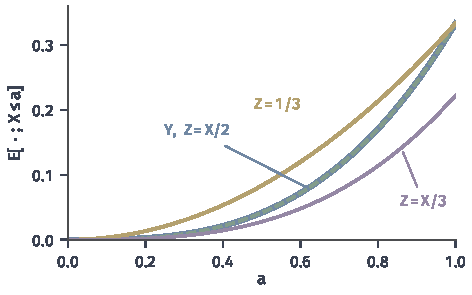
\includegraphics[width=80mm]{figures/07-probability/02-measure-theoretic-probability/matplotlib/cexp-cumulative-check/figure.pdf}
  \caption{用积分刻画检验候选，三角形模型。横轴为$a$，纵轴为事件$\{X\leq a\}$上的累计期望。蓝线是$Y$的$a^{3}/3$，绿色虚线是候选$Z=X/2$，两者重合；黄线是常数候选$1/3$，紫线是候选$X/3$，都与蓝线分离。}
  \label{fig:cexp-cumulative-check}
\end{BookInlineFigure}

\subsection{存在性与唯一性}
\label{sec:cexp-existence}

定义只列出要求，还没有说明满足要求的随机变量是否存在、有几个。有限划分时，式~\eqref{eq:cexp-partition}给出了一个解，零概率组上的任意取值又说明解可能不止一个。一般的$\mathcal{G}$没有组可以逐个处理，需要另找办法。

\paragraph{累计期望是一个测度}
关键是换一个角度看式~\eqref{eq:cexp-defining}的右边。先设$X\geq0$且可积，对$A\in\mathcal{G}$令
\[
 \nu(A)=\mathbb{E}[X\mathbf{1}_{A}] .
\]
$\nu$把每个已知事件对应到$X$在其上的累计期望，可以想成把“$X$的质量”分配到已知事件上。式~\eqref{eq:cexp-defining}要求找一个$\mathcal{G}$可测的$Z$，使$\nu(A)=\mathbb{E}[Z\mathbf{1}_A]$：$Z$是$\nu$相对于$\mathbb{P}$的密度，而且这个密度只能用$\mathcal{G}$中的信息。卷四的Radon--Nikodym定理回答的正是这样的问题：$\sigma$有限测度$\nu$关于$\mu$绝对连续时，存在非负可测函数$h$，使$\nu(A)=\int_A h\,\mathrm{d}\mu$对一切可测集成立，并且$h$在$\mu$几乎处处的意义下唯一，可参考\BookChapterRef{chap:measure-densities}{卷四第8章“测度的密度”}。

图~\ref{fig:cexp-rn-cumulative}用逐次等分的例子展示这个视角。在整个$\mathcal{F}$上，
\[
 \nu([0,t))=\int_0^t\omega^{2}\,\mathrm{d}\omega=\frac{t^{3}}{3},
\]
这条蓝色曲线的斜率就是$X$本身：在$\mathcal{F}$上，$\nu$的密度是$X$。若只允许使用$\mathcal{G}_2$中的事件，$\nu$只在四段及其并上有定义，四段上的质量是
\[
 \begin{gathered}
 \nu(A_1)=\tfrac{1}{192},\qquad \nu(A_2)=\tfrac{7}{192},\\ \nu(A_3)=\tfrac{19}{192},\qquad \nu(A_4)=\tfrac{37}{192},
 \end{gathered}
\]
其中$A_1,\dots,A_4$依次是四个区间。$\mathcal{G}_2$可测的密度在每段上只能取常数，它在$A_i$上必须等于比值$\nu(A_i)/\mathbb{P}(A_i)$，也就是折线在各段的斜率$1/48$、$7/48$、$19/48$、$37/48$，正是第~\ref{sec:cexp-finite-partition}节算出的条件平均。

\begin{BookInlineFigure}
  \centering
  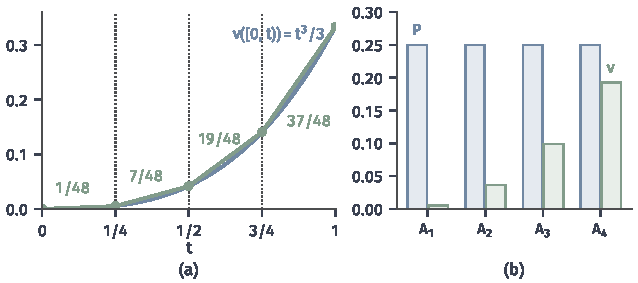
\includegraphics[width=108mm]{figures/07-probability/02-measure-theoretic-probability/matplotlib/cexp-rn-cumulative/figure.pdf}
  \caption{条件期望是限制在$\mathcal{G}$上的密度，$\Omega=[0,1)$，$X(\omega)=\omega^{2}$，$\mathcal{G}=\mathcal{G}_2$。(a)蓝线是$\nu([0,t))=t^{3}/3$，斜率为$X$；绿色折线只经过四个分点，各段斜率是$\mathbb{E}[X\mid\mathcal{G}_2]$的取值。(b)四个区间上$\mathbb{P}(A_i)=1/4$（蓝）与$\nu(A_i)$（绿）的比较，两者之比就是各段斜率。}
  \label{fig:cexp-rn-cumulative}
\end{BookInlineFigure}

\paragraph{存在与唯一}
有了这个视角，存在性归结为在可测空间$(\Omega,\mathcal{G})$上使用Radon--Nikodym定理。唯一性则只用到式~\eqref{eq:cexp-defining}对足够多的事件成立。

\begin{theorem}[条件期望的存在与唯一]
\label{thm:cexp-existence}
设$X$可积，$\mathcal{G}\subseteq\mathcal{F}$是$\sigma$代数。则$X$给定$\mathcal{G}$的条件期望存在。若$Z$与$Z'$都是它的版本，则$Z=Z'$几乎必然成立；反过来，若$Z$是一个版本，$Z'$是$\mathcal{G}$可测的随机变量且$Z'=Z$几乎必然成立，则$Z'$也是一个版本。
\end{theorem}

\begin{proof}
\emph{第一步，非负的$X$。}设$X\geq0$且可积，对$A\in\mathcal{G}$令$\nu(A)=\mathbb{E}[X\mathbf{1}_{A}]$。$\nu(\emptyset)=0$；若$A_1,A_2,\dots\in\mathcal{G}$两两不交，则
\[
 X\mathbf{1}_{\bigcup_nA_n}=\sum_nX\mathbf{1}_{A_n},
\]
右边各项非负，由单调收敛定理，
\[
 \nu\Bigl(\bigcup_nA_n\Bigr)=\sum_n\nu(A_n).
\]
所以$\nu$是$(\Omega,\mathcal{G})$上的测度，总质量$\nu(\Omega)=\mathbb{E}[X]<\infty$。

记$\mathbb{P}_{\mathcal{G}}$为$\mathbb{P}$限制在$\mathcal{G}$上得到的概率测度。若$A\in\mathcal{G}$且$\mathbb{P}(A)=0$，则$X\mathbf{1}_{A}$只在零概率集上非零，$\nu(A)=0$，即$\nu\ll\mathbb{P}_{\mathcal{G}}$。两个测度都有限，由Radon--Nikodym定理，存在$\mathcal{G}$可测的$Z:\Omega\to[0,\infty)$，使
\[
 \nu(A)=\int_{A}Z\,\mathrm{d}\mathbb{P}_{\mathcal{G}},\qquad A\in\mathcal{G}.
\]

右边是对$\mathbb{P}_{\mathcal{G}}$的积分，需要把它换成对$\mathbb{P}$的积分。对$\mathcal{G}$中事件的示性函数，两者都是$\mathbb{P}(A)$；由线性，对$\mathcal{G}$可测的非负简单函数两者相等；非负$\mathcal{G}$可测函数可以由这样的简单函数单调逼近，由单调收敛定理两者仍相等。于是
\[
 \mathbb{E}[Z\mathbf{1}_{A}]=\nu(A)=\mathbb{E}[X\mathbf{1}_{A}],\qquad A\in\mathcal{G}.
\]
取$A=\Omega$得$\mathbb{E}[Z]=\mathbb{E}[X]<\infty$，$Z$可积。$Z$满足定义的三条要求。

\emph{第二步，一般的$X$。}把$X$拆成$X=X^{+}-X^{-}$，两部分非负且可积。由第一步取版本$Z_{+}$与$Z_{-}$，令$Z=Z_{+}-Z_{-}$。它是$\mathcal{G}$可测且可积的，对$A\in\mathcal{G}$，由期望的线性，
\[
 \mathbb{E}[Z\mathbf{1}_{A}]=\mathbb{E}[X^{+}\mathbf{1}_{A}]-\mathbb{E}[X^{-}\mathbf{1}_{A}]=\mathbb{E}[X\mathbf{1}_{A}] .
\]

\emph{第三步，唯一性。}设$Z,Z'$都是版本。两者都$\mathcal{G}$可测，所以$A=\{Z>Z'\}\in\mathcal{G}$。由式~\eqref{eq:cexp-defining}，
\[
 \mathbb{E}\bigl[(Z-Z')\mathbf{1}_{A}\bigr]=\mathbb{E}[X\mathbf{1}_{A}]-\mathbb{E}[X\mathbf{1}_{A}]=0 .
\]
被积函数$(Z-Z')\mathbf{1}_{A}$非负而期望为零，所以它几乎必然为零；它在$A$上严格为正，于是$\mathbb{P}(A)=0$。交换$Z$与$Z'$得$\mathbb{P}(Z'>Z)=0$，所以$Z=Z'$几乎必然成立。

最后，若$Z'$是$\mathcal{G}$可测的且$Z'=Z$几乎必然成立，则$Z'$可积，并且对每个$A$，$Z'\mathbf{1}_{A}$与$Z\mathbf{1}_{A}$几乎必然相等，期望相同，所以$Z'$也满足式~\eqref{eq:cexp-defining}。
\end{proof}

\paragraph{版本与几乎必然}
定理说明，条件期望是一个只确定到零概率集的对象：不同版本可以在一个零概率集上取不同的值，除此之外完全一样。这与有限划分中零概率组上的任意常数是同一回事。所以，凡是关于$\mathbb{E}[X\mid\mathcal{G}]$的等式和不等式，都按几乎必然的意义理解，并且对它的任何一个版本都成立；后文不再逐次声明。

修改一个版本时要注意可测性。改动后的随机变量必须仍是$\mathcal{G}$可测的；若$\mathcal{G}$不含某个零概率集的全部子集，在其上随意改值可能破坏这一点，这时定理的最后一句不能使用。第~\ref{chap:probability-spaces}章的完备化可以消除这类麻烦，但条件期望的定义并不依赖它。

第~\ref{sec:cexp-prediction}节还会给出另一条构造路线：当$X$平方可积时，条件期望是一个正交投影。那条路线只适用于平方可积的变量，一般的可积变量仍由上面的定理保证。

\subsection{给定随机变量的条件期望}
\label{sec:cexp-given-variable}

\paragraph{给定观测的条件期望}
最常见的信息来自一个观测。设$Y$是取值于$\mathbb{R}^{k}$的随机向量，或者更一般地，取值于某个可测空间$(E,\mathcal{E})$的随机对象。第~\ref{chap:probability-spaces}章定义了它生成的$\sigma$代数
\[
 \sigma(Y)=\bigl\{\{Y\in B\}:\ B\in\mathcal{E}\bigr\},
\]
它由所有“能凭$Y$的值判断是否发生”的事件组成。对可积的$X$，定义
\begin{equation}
 \mathbb{E}[X\mid Y]=\mathbb{E}\bigl[X\mid\sigma(Y)\bigr].
 \label{eq:cexp-given-variable}
\end{equation}
给定几个观测$Y_1,\dots,Y_k$时，把它们合成一个随机向量$(Y_1,\dots,Y_k)$。

在传感器表中，$\mathbb{E}[Y\mid X]=m(X)$是$X$的函数。一般情形下，$\sigma(Y)$可测的随机变量是否也都能写成$Y$的函数？直观上应当如此：$\sigma(Y)$可测意味着样本点只要$Y$值相同，取值就相同，见图~\ref{fig:cexp-factorization}。下面的\term{因子分解引理}（factorization lemma）把这一点写准。

\begin{BookInlineFigure}
  \centering
  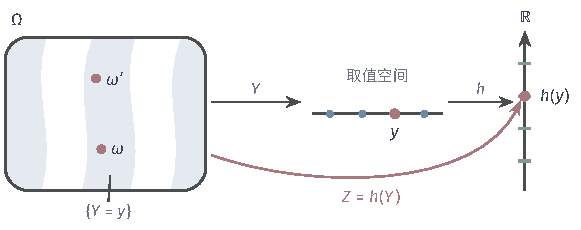
\includegraphics[width=98mm]{figures/07-probability/02-measure-theoretic-probability/tikz/cexp-factorization/figure.pdf}
  \caption{经由观测的因子分解。左边$\Omega$被分成水平集$\{Y=y\}$（浅蓝与白色条带）；同一条带内的$\omega$与$\omega'$有相同的$Y$值，因而$\sigma(Y)$可测的$Z$在两点取值相同。于是$Z$可以先经$Y$映到取值空间，再经可测函数$h$映到$\mathbb{R}$，即$Z=h(Y)$。}
  \label{fig:cexp-factorization}
\end{BookInlineFigure}

\begin{lemma}[因子分解引理]
\label{lem:cexp-factorization}
设$Y:\Omega\to E$关于$\mathcal{E}$可测，$Z:\Omega\to\mathbb{R}$关于$\sigma(Y)$可测。则存在可测函数$h:E\to\mathbb{R}$，使$Z=h(Y)$在$\Omega$上处处成立。
\end{lemma}

\begin{proof}
先设$Z$是示性函数$\mathbf{1}_{A}$，$A\in\sigma(Y)$。由$\sigma(Y)$的定义，有$B\in\mathcal{E}$使$A=\{Y\in B\}$，于是
\[
 Z=\mathbf{1}_{B}(Y),
\]
取$h=\mathbf{1}_{B}$即可。若$Z$是有限个这样的示性函数的线性组合$\sum_{i}a_i\mathbf{1}_{A_i}$，对每个$A_i$取对应的$B_i$，令$h=\sum_ia_i\mathbf{1}_{B_i}$。

一般情形，取$\sigma(Y)$可测的简单函数$Z_n$，使$Z_n(\omega)\to Z(\omega)$对每个$\omega$成立；例如把$\max(-n,\min(Z,n))$向零截断到$2^{-n}$的整数倍。由上一段，$Z_n=h_n(Y)$，$h_n$可测。令
\[
 L=\bigl\{e\in E:\ \lim_{n\to\infty}h_n(e)\ \text{存在且有限}\bigr\},
\]
它是$\limsup_nh_n$与$\liminf_nh_n$相等且有限的点集，因而可测；在$L$上令$h=\lim_nh_n$，在$L$外令$h=0$，$h$可测。对每个$\omega$，数列$h_n(Y(\omega))=Z_n(\omega)$收敛到$Z(\omega)$，所以$Y(\omega)\in L$，并且$h(Y(\omega))=Z(\omega)$。
\end{proof}

把引理用于$\mathbb{E}[X\mid Y]$的任一版本，得到可测函数$m:E\to\mathbb{R}$，使
\begin{equation}
 \mathbb{E}[X\mid Y]=m(Y).
 \label{eq:cexp-regression-function}
\end{equation}
按惯例记$\mathbb{E}[X\mid Y=y]=m(y)$。由于$\sigma(Y)$中的事件都是$\{Y\in B\}$，并且$\mathbb{E}[m(Y)\mathbf{1}_B(Y)]$可以用推前分布写成对$P_Y$的积分，一个可测函数$m$满足要求，当且仅当$m(Y)$可积，并且对每个$B\in\mathcal{E}$，
\begin{equation}
 \mathbb{E}\bigl[X\mathbf{1}_{\{Y\in B\}}\bigr]=\int_{B}m(y)\,P_Y(\mathrm{d}y).
 \label{eq:cexp-given-variable-check}
\end{equation}

\paragraph{函数只在分布下几乎处处确定}
$m(Y)$与$m(y)$要分清。前者是$\Omega$上的随机变量，作为条件期望的版本，几乎必然唯一；后者是取值空间上的普通函数。两个函数$m,\tilde m$都满足要求，当且仅当$m(Y)=\tilde m(Y)$几乎必然成立，也就是
\[
 P_Y\bigl(\{y:\ m(y)\neq\tilde m(y)\}\bigr)=\mathbb{P}\bigl(m(Y)\neq\tilde m(Y)\bigr)=0 .
\]
所以$m$只在$P_Y$几乎处处的意义下确定：在$Y$取不到的地方，$m$可以任意取值；在$Y$以零概率取到的单个点上，$m$的值也没有意义。

“只知绝对值”的例子把这一点画得很清楚。$Y=\lvert X\rvert\sim\operatorname{Unif}(0,1)$，$m(y)=y/2$是$\mathbb{E}[X^{+}\mid Y=y]$的一个版本。把$m$在$y=1/2$处改成$0.9$，并在$[0,1]$之外任意改动，得到的$\tilde m$仍是一个版本，见图~\ref{fig:cexp-versions}(a)。在$\Omega$上看，$\tilde m(Y)$与$m(Y)$只在$\omega=\pm1/2$两点不同，见图~\ref{fig:cexp-versions}(b)。问“已知$\lvert X\rvert=1/2$时$X^{+}$的平均是多少”，单凭条件期望的定义无法回答；要给单个观测值指定确定的条件平均，需要额外的要求，例如$m$的连续性，这在第~\ref{chap:conditional-distributions}章讨论。

\begin{BookInlineFigure}
  \centering
  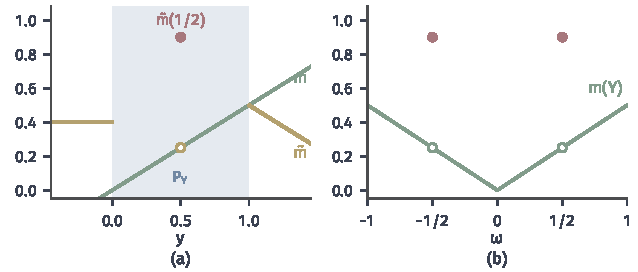
\includegraphics[width=108mm]{figures/07-probability/02-measure-theoretic-probability/matplotlib/cexp-versions/figure.pdf}
  \caption{$\mathbb{E}[X^{+}\mid Y]$的两个版本，$Y=\lvert X\rvert$，$X\sim\operatorname{Unif}(-1,1)$。(a)绿线$m(y)=y/2$；黄线与红点组成的$\tilde m$在$[0,1]$上只在$y=1/2$处不同，在浅蓝区间$[0,1]$（$P_Y$所在之处）以外任意取值。(b)复合到$\Omega$上，$\tilde m(Y)$与$m(Y)$只在$\omega=\pm1/2$两点（红点）不同。}
  \label{fig:cexp-versions}
\end{BookInlineFigure}

\paragraph{回到条件均值的公式}
式~\eqref{eq:cexp-given-variable-check}说明，第~\ref{chap:random-vectors}章的两个公式都给出了版本。若$Y$只取可数多个值，对$\mathbb{P}(Y=y)>0$的$y$令
\[
 m(y)=\frac{\mathbb{E}\bigl[X\mathbf{1}_{\{Y=y\}}\bigr]}{\mathbb{P}(Y=y)},
\]
其余$y$上任意取值。两边对$B$中的$y$求和，式~\eqref{eq:cexp-given-variable-check}成立，交换求和与期望由$\mathbb{E}\lvert X\rvert<\infty$保证。

若$(X,Y)$有联合密度$f_{X,Y}$，$Y$为实值，在$f_Y(y)>0$处令
\[
 m(y)=\frac{1}{f_Y(y)}\int x\,f_{X,Y}(x,y)\,\mathrm{d}x ,
\]
其余$y$上令$m(y)=0$。由$\mathbb{E}\lvert X\rvert<\infty$与Fubini定理，
\[
 \mathbb{E}\bigl[X\mathbf{1}_{\{Y\in B\}}\bigr]=\int_{B}\int x\,f_{X,Y}(x,y)\,\mathrm{d}x\,\mathrm{d}y=\int_{B}m(y)f_Y(y)\,\mathrm{d}y ,
\]
这正是式~\eqref{eq:cexp-given-variable-check}。$f_Y(y)=0$的那些$y$对右边没有贡献，$m$在那里怎样取都可以。

没有密度时，可以像前面那样直接验证候选。在“只知绝对值”的例子中，对满足$\mathbb{E}\lvert g(X)\rvert<\infty$的可测函数$g$，把积分按$\pm x$配对，
\[
 \mathbb{E}\bigl[g(X)\mathbf{1}_{\{Y\in B\}}\bigr]
 =\int_{0}^{1}\frac{g(y)+g(-y)}{2}\,\mathbf{1}_{B}(y)\,\mathrm{d}y .
\]
右边正是式~\eqref{eq:cexp-given-variable-check}，其中$P_Y$是$[0,1]$上的均匀分布，所以
\begin{equation}
 \mathbb{E}\bigl[g(X)\bigm|\lvert X\rvert\bigr]=\frac{g(\lvert X\rvert)+g(-\lvert X\rvert)}{2}.
 \label{eq:cexp-folding}
\end{equation}
取$g(x)=x^{+}$得到$\lvert X\rvert/2$；取$g(x)=x$得到$0$；取$g(x)=\mathrm{e}^{x}$得到$\cosh\lvert X\rvert$，见图~\ref{fig:cexp-folding}(b)。
